\documentclass[english,11pt,a4paper]{article}
\usepackage[margin=1in]{geometry}
\usepackage{fontspec}
\setmainfont{lmroman10-regular.otf}[BoldFont=lmroman10-bold.otf,ItalicFont=lmroman10-italic.otf,BoldItalicFont=lmroman10-bolditalic.otf]
\setsansfont{lmsans10-regular.otf}[BoldFont=lmsans10-bold.otf]
\setmonofont{lmmono10-regular.otf}[Scale=MatchLowercase]
\newlength{\LeanCharWidth}
\usepackage{amsmath,amssymb}
\usepackage[english]{babel}
\usepackage{microtype,parskip}
\usepackage{graphicx,float,caption}
\usepackage{longtable,booktabs,array,calc}
\usepackage{xcolor}
\usepackage{xurl}
\usepackage{hyperref,bookmark}
\usepackage{etoolbox,needspace}
\setcounter{secnumdepth}{-\maxdimen}
\setlength{\emergencystretch}{3em}
\providecommand{\tightlist}{\setlength{\itemsep}{0pt}\setlength{\parskip}{0pt}}
\newcounter{none}
\AtBeginEnvironment{longtable}{\Needspace{8\baselineskip}\small}
\pretocmd{\section}{\Needspace{5\baselineskip}}{}{}
\pretocmd{\subsection}{\Needspace{4\baselineskip}}{}{}
\pretocmd{\subsubsection}{\Needspace{4\baselineskip}}{}{}
\captionsetup{font=small,labelfont=bf}
\urlstyle{same}
\AtBeginDocument{\special{pdf:minorversion 7}}

\hypersetup{pdflang=en-US,colorlinks=true,urlcolor=blue,linkcolor=blue,pdftitle={Recovering Host-Triangle Decompositions after Random Deletions in Split Graphs},pdfauthor={Juan Pablo Traverso Gianini}}
\title{Recovering Host-Triangle Decompositions after Random Deletions in Split Graphs}
\author{Juan Pablo Traverso Gianini\\\small Independent researcher, Santiago, Chile\\\small\href{mailto:jtraverso@gmail.com}{jtraverso@gmail.com}\quad\href{https://orcid.org/0009-0003-6068-4096}{ORCID 0009-0003-6068-4096}}
\date{Preprint 1.0 \enspace·\enspace November 24, 2026}
\begin{document}\raggedbottom\maketitle
\begin{center}Paper III in the series on clique partition gaps in split graphs.\end{center}
\noindent DOI \url{https://doi.org/10.5281/zenodo.24494747}\\
Series repository \url{https://github.com/jtraverso/split-clique-partition-gap}
\subsection{Abstract}\label{abstract}

We retain each core--host incidence independently with probability \(p\). When the required pairs form \(K_d\) or \(K_{d,d}\) and \(\lceil Kd\rceil\) hosts are available with \(Kp>1\), we show that with high probability the surviving incidences contain a balanced support satisfying the four hypotheses of physical typed absorption. On this support a single decomposition uses every required pair and every selected crossing edge exactly once.

For every fixed \(0<p<1\) and all sufficiently large \(n\), the construction gives an \(n\)-vertex split graph whose nearly quadratic clique-partition gap survives deletion exactly with high probability. On the same event the graph retains linear vertex connectivity. One assignment approximates the prescribed bounded linear statistics and Pasch counts to within \(o(n^2)\) across the whole graph and \(o(t^2)\) on triangles with bases in the original geometric core of \(15t\) vertices. The triangles assigned to bases in the original core contain \((225p^2/8+o(1))t^2\) Pasch configurations. For general request graphs of maximum degree \(d\) and polynomial order, weighted list edge-coloring gives the sharp uniform recovery condition \(Kp>1\) for \(\lceil Kd\rceil\) hosts.

\subsection{1. Reconstruction, prescribed statistics and the clique-partition gap}\label{reconstruction-prescribed-statistics-and-the-clique-partition-gap}

In a split graph the core vertices form a clique and the remaining vertices form an independent set. Every clique that meets the independent set contains just one of its vertices, which we call its \emph{host}. Part I, \emph{Nearly Quadratic Additive Gaps for Edge-Clique Partitions of Split Graphs} {[}1{]}, used host triangles to realize a packing problem on the core. Part II, \emph{Stability of the Clique Partition Gap in Split Graphs} {[}2{]}, showed that losing \(L\) assignments changes the comparison with that packing problem by at most \(2L\). Its construction allowing quadratically many deletions protected the assigned triangles on the original core. Here both crossing edges of every assigned triangle are subject to deletion. A pair whose triangle is lost may still have another common host. To recover all pairs at once, the replacement triangles must use distinct crossing edges.

A \emph{base} is a required pair of core vertices. Assigning it to a common host produces a triangle whose two crossing edges join its endpoints to that host. An assignment is \emph{proper} if the bases assigned to each host form a matching. In our construction, any complete proper assignment preserves the clique-partition gap. Prescribing statistics also constrains the choice of its triangles. A Pasch consists of four triangles on six vertices, with each vertex occurring twice and no two triangles sharing an edge.

Write \(\operatorname{cp}(G)\) for the minimum number of cliques in a partition of the edges of \(G\). Its fractional counterpart \(\operatorname{cp}^{\ast}(G)\) minimizes the sum of nonnegative clique weights subject to total weight one on every edge. Cliques may have any order at least two. We write \(\Delta(G)=\operatorname{cp}(G)-\operatorname{cp}^{\ast}(G)\), and \(\kappa(G)\) for vertex connectivity. For the remainder of the paper \(p\) denotes the probability that a crossing edge \emph{survives}. All core edges remain present. Logarithms are natural.

\textbf{Theorem 1 (reconstruction of a balanced support).} Fix \(0<p<1\) and \(K>1/p\). There are constants \(C\ge1\), \(\alpha>0\) and \(\eta_0>0\), with \(\eta_0<Kp-1\), for which the following holds. For every fixed \(0<\eta<\eta_0\) there are \(c>0\) and \(d_0\) such that, for \(d\ge d_0\), we may start with either \(K_{d,d}\) or \(K_d\) as the graph of bases and prescribe any \(r=\lceil(1+\eta)d/p\rceil\) of the \(\lceil Kd\rceil\) available hosts before deletion. Independently retain each crossing incidence with probability \(p\). With probability at least \(1-\exp(-c d^{1/3})\) there exists a graph \(H\) on the core and these \(r\) hosts whose edges are all the bases together with a subset of the surviving crossing edges. Write \(N=|V(H)|\). The allowed triangle types are (left, right, host) in the bipartite case and (core, core, host) in the clique case. The following four properties hold on this same \(H\).

\begin{enumerate}
\def\labelenumi{\arabic{enumi}.}
\tightlist
\item
  \textbf{Diffuse seed (H1).} Every allowed triangle \(T\) has a weight \(\mu_T\in[1/(CN),C/N]\), and the weights at each edge of \(H\) sum to one.
\item
  \textbf{Integer certificate (H2).} The edge indicator of \(H\) is an integer linear combination of the indicators of its allowed triangles.
\item
  \textbf{Common neighbors (H3).} For every two distinct vertices and every label that completes their labels to an allowed type, at least \(\alpha N\) common neighbors have that label. This includes nonadjacent pairs.
\item
  \textbf{Physical hinges (H4).} For allowed triangles \(uvx,uvy\) with \(x\ne y\), there are at least \(\alpha N^2\) distinct sets of auxiliary edges \(J\subseteq E(H)\) incident with exactly six vertices and edge-disjoint from both root triangles. Each of \(J\cup\{ux,vx\}\) and \(J\cup\{uy,vy\}\) has a decomposition into allowed triangles.
\end{enumerate}

For an initial pool of \(r\) hosts at a base \(e\), give each of its \(r\) candidate triangles weight \(\lambda_T=1/r\). These weights describe the choice of a host uniformly for each base before we know anything about survival. Write \(\mathcal C\) for these candidates, restricted to the pool designated for each base. For a real test \(f\) on \(\mathcal C\) and for the set \(\mathcal P(\mathcal C)\) of its unordered Pasch configurations, the two target values are

\[M_\lambda(f)=\sum_{T\in\mathcal C} f(T)\lambda_T,\qquad
P_\lambda=\sum_{P\in\mathcal P(\mathcal C)}\prod_{T\in P}\lambda_T.
\tag{1}\]

For example, taking \(f\) to be the indicator of triangles using a specified set of hosts measures their share of the final assignment. Formula (1) also makes sense for a signed test.

\textbf{Theorem 2 (statistics on two scales).} For fixed \(0<p<1\) there is a sequence of split graphs of every sufficiently large order \(n\) satisfying Theorem 3 below. Each has an original core \(U\) of \(15t\) vertices, with \(t=\Theta_p(n/\sqrt{\log n})\), and initial host pools chosen before deletion. The graph sequence and its pools work for every fixed \(q\ge0\). Given a family \(\mathcal F_n\) of at most \(n^q\) tests \(|f|\le1\) chosen before deletion, with probability tending to one there exists a complete proper assignment \(\mathcal D\) on the surviving graph for which \[\max_{f\in\mathcal F_n}\left|\sum_{T\in\mathcal D}f(T)-M_\lambda(f)\right|=o(n^2),
\qquad |P(\mathcal D)-P_\lambda|=o(n^2).
\tag{2}\]

Write \(\mathcal D_U\) and \(\mathcal C_U\) for the assigned and candidate triangles whose two core vertices are in \(U\). Use the same weights in (1), restricted to \(\mathcal C_U\), to define \(M_{\lambda,U}\) and \(P_{\lambda,U}\). The same assignment satisfies \[\max_{f\in\mathcal F_n}\left|\sum_{T\in\mathcal D_U}f(T)-M_{\lambda,U}(f)\right|=o(t^2),
\qquad |P(\mathcal D_U)-P_{\lambda,U}|=o(t^2).
\tag{3}\]

When the family is empty, the bounds on tests are vacuous. Every base and every crossing edge of the selected support belongs to exactly one triangle of \(\mathcal D\). With \(|W|\sim p^2n/64\) additional core vertices, the two counts are \[P(\mathcal D)=\frac{p^6}{32768}\,n^2+o(n^2),
\qquad
P(\mathcal D_U)=\frac{225p^2}{8}\,t^2+o(t^2).
\tag{4}\]

\textbf{Theorem 3 (gap and connectivity).} Fix \(0<p<1\). There are constants \(a_p,c_p>0\) such that for every sufficiently large \(n\) there is an \(n\)-vertex split graph \(G_n\) with

\[\Delta(G_n)\ \ge\ a_p\,\frac{n^2}{(\log n)^{5/2}}
  \exp\!\left(-2\sqrt{\log(24/7)\log n}\right).
\tag{5}\]

Let \(G'_n\) be obtained by retaining each crossing edge independently with probability \(p\). Then

\[\Pr\!\left(\Delta(G'_n)=\Delta(G_n)
             \ \text{and}\ \kappa(G'_n)\ge c_p n\right)\longrightarrow 1.
\tag{6}\]

Balogh, He, Krueger, Nguyen and Wigal {[}7, Theorem 1.10{]} give \(\Delta(G)=o(n^2)\) for general graphs upon setting \(t=2\) and assigning unit clique costs in their decomposition theorem. The lower bound (5) is of order \(n^{2-o(1)}\) within this subquadratic range. For a particular triangle designated before deletion, the probability that both crossing edges survive is only \(p^2\). Under the neighborhood independence condition below, every complete proper assignment of the same required pairs realizes the same packing gap. We recall the precise statement from {[}1, Lemma 2.1{]} and {[}2, Lemma 2{]}.

Let \(V\) denote the core and let \(B\) be a graph on \(V\), called the \emph{residual graph}. The required pairs are \(J=\binom V2\setminus E(B)\). For a core set \(Q\) of order at least two, its residual score is

\[w_B(Q)=\binom{|Q|}{2}-1-2\left|J\cap\binom Q2\right|.\]

The first two terms give the saving over single edges from using \(Q\) as a clique. Each required pair occupied by \(Q\) displaces a potential host triangle, whose saving is two. Write \(I(B)\) for the maximum total score over families of core sets using each pair at most once. The fractional maximum \(F(B)\) allows a nonnegative weight on each set and imposes the same unit capacity on every pair. Put \(\Phi(B)=F(B)-I(B)\).

The triangles of a proper host assignment are edge-disjoint. If every host neighborhood is independent in \(B\) and there is a proper assignment of all of \(J\), the exact transfer identities give

\[\operatorname{cp}(G)=|E(G)|-2|J|-I(B),\qquad
\operatorname{cp}^{\ast}(G)=|E(G)|-2|J|-F(B).
\tag{7}\]

The term containing \(|E(G)|\) cancels on subtraction. Deletions can shrink a host neighborhood while preserving its independence in \(B\). Thus, to obtain the same gap after deletion, it suffices to assign the same required pairs again. Section 2 proves recovery for one pool of hosts. In Sections 3--4 we give every required pair of Part I a designated block. Sections 5--6 reconstruct the balanced support and control the statistics of a single decomposition on both scales.

\subsection{2. Recovery from random host lists}\label{recovery-from-random-host-lists}

Let \(R\) be a finite simple graph of requests. Each host initially sees all vertices of \(R\). After deletion, each edge \(uv\) of \(R\) has a list consisting of the hosts that still see both \(u\) and \(v\). These lists are dependent. For example, loss of the incidence \(hu\) removes \(h\) from every list at \(u\). The following result uses precisely this incidence model. We write \(d\) for the maximum degree of \(R\) to distinguish it from the partition gap.

\textbf{Theorem 4 (recovery from random host lists).} Fix \(p\in(0,1)\), \(K>1/p\) and \(A\ge1\). Suppose \(R\) has maximum degree \(d\) and at most \((d+1)^A\) vertices. Equip \(R\) with \(\lceil Kd\rceil\) hosts, retaining each vertex--host incidence independently with probability \(p\). For all sufficiently large \(d\), a proper assignment covers every edge of \(R\) except on an event of probability at most \(C d^{C}\exp(-c\sqrt d)\), for constants \(C,c>0\) depending only on \(p,K,A\). For \(K>0\) with \(Kp\le1\), a uniform high-probability conclusion fails even on \(K_{d+1}\), which belongs to the stated size class for every \(A\ge1\).

\emph{Proof.} A vertex of degree \(d\) must see at least \(d\) distinct hosts. If \(Kp<1\), its surviving count is a binomial random variable with mean at most \(Kpd+1\) and falls short with probability tending to one. When \(Kp=1\), the complete graph \(R=K_{d+1}\) gives the obstruction. Each vertex sees a binomially distributed number of hosts with mean \(d+O(1)\) and variance of order \(d\). By the central limit theorem its probability of seeing fewer than \(d\) tends to \(1/2\). The counts at different vertices use disjoint incidences. Hence with probability tending to one some vertex falls short.

Suppose now that \(Kp>1\) and put \(m=\lceil Kd\rceil\). For a request \(e=uv\) let \(L(e)\) be its surviving list, and let \(Z(u,h)\) count the requests at \(u\) whose list contains \(h\). The list size has distribution \(\mathrm{Bin}(m,p^2)\). Conditional on \(hu\) surviving, \(Z(u,h)\) has distribution \(\mathrm{Bin}(\deg_R(u),p)\), since the other endpoints of these requests are distinct. Otherwise \(Z(u,h)=0\). Chernoff's inequality, followed by a union bound over at most \(d(d+1)^A/2\) requests and \(m(d+1)^A\) incidences, gives \[|L(e)|\ge mp^2-d^{3/4},\qquad Z(u,h)\le pd+d^{3/4}
 \tag{8}\] simultaneously, except with probability \(d^{O(1)}\exp(-\Omega_{p,K}(\sqrt d))\).

Put \(b=\lceil pd+d^{3/4}\rceil\) and give each available host color weight \(1/b\). At an endpoint \(u\), the competing edges with a given color \(h\) have total weight at most \(Z(u,h)/b\le1\). Each list has total weight at least \((mp^2-d^{3/4})/b\), which tends to \(Kp\). For large \(d\) this is at least \(1+(Kp-1)/2\). The individual weights satisfy \(\exp(-b^{1/25})\le1/b\). These are the weight, list-mass and conflict bounds in the theorem of Bonamy, Delcourt, Lang and Postle {[}3, Theorem 6{]}, applied with parameter \(b\) to the simple graph \(R\). A proper list edge-coloring gives the required assignment on the event (8). \(\square\)

In the random-list models studied by Jain and Pham {[}8{]} and Keevash {[}10{]}, colors are sampled for the edges of the request graph. In our model the independent trials are the vertex--host incidences. The loss of \(hu\) removes \(h\) from every list at \(u\) at once. Conditioning on the survival of \(hu\) gives the local conflict bound required by the coloring theorem.

\subsection{3. A pool for every required core pair}\label{a-pool-for-every-required-core-pair}

We use the following data from the construction in {[}1, §§4--6{]}. Its fifteen roles come in three color classes, five roles in each. In each role the positions are the elements of

\[D_m=(\mathbb Z/m\mathbb Z)^2,\qquad T=D_m^j,\qquad t=|T|=m^{2j},\]

where \(m\) is odd and \(j\ge2\). Of the pairs of roles, counting a repeated role once, 54 are edges of the fifteen-role graph. For such a pair, let \(b\in\{1,2\}\) be the difference of its color indices, in increasing order. The core pair with positions \(x,y\) is an edge of \(B\) exactly when its direction \((y-x)/b\) lies in \(S_m^j\), for the set \(S_m\subset D_m\) of {[}1{]}. For each of the 66 other role types all pairs of distinct vertices are required. The only geometric property of \(S_m\) used to construct hosts is that its complement has a partition into at most 24 classes \(C\) such that

\[u,v\in C\quad\Longrightarrow\quad (u+v)/2\notin S_m.
\tag{9}\]

Division by two is well defined because \(m\) is odd. The quantitative packing bound for this specific \(S_m\) enters in Section 4.

To count the available hosts for a pair, fix a set of directions \(U\subset T\) and a center \(z\in T\). A host sees the positions \(z-bU/2\) in the first role and \(z+bU/2\) in the second. For the pair \((x,x+ba)\) of direction \(a\), put \(u=2(z-x)/b\). The first membership condition is \(u\in U\), and the second, \(x+ba\in z+bU/2\), is equivalent to \(2a-u\in U\). Thus the number of centers serving this pair is exactly \(|U\cap(2a-U)|\). Specifying a class down to the last coordinate can leave very few centers. If one coordinate is unrestricted, varying that coordinate of the center gives at least \(m^2\) interchangeable choices for every pair designated to the class.

\textbf{Lemma 5 (two orders of the coordinates).} For an integer \(K\ge1\), the required pairs in the 54 role types admit a system of at most \(1296Kjt\) hosts with neighborhoods independent in \(B\). Each required pair is assigned to one auxiliary complete bipartite graph \(K_{d,d}\) with \(d\ge m^2\) and \(Kd\) available hosts. Two auxiliary graphs using the same hosts have disjoint vertex sets. On restricting each assignment to its designated pairs, proper assignments on all the auxiliary graphs give a proper assignment of all the required pairs of these types.

\emph{Proof.} \emph{Ownership of a direction.} In the order \(1,\ldots,j\), use the first coordinate outside \(S_m\) whenever it occurs among the first \(j-1\). If all those coordinates lie in \(S_m\), the last one must lie outside. In that case read the coordinates in the order \(1,\ldots,j-2,j,j-1\). The failed coordinate is now followed by the original penultimate coordinate. For instance, with three coordinates a direction in \(S_m\times S_m\times C\) is handled in order \(1,3,2\), leaving coordinate 2 free. The two rules assign every required direction exactly once.

\[\begin{array}{c|ccc|c}
 &\text{common prefix}&\text{next coordinate}&\text{free coordinate}&\text{block size}\\ \hline
 \text{primary}&1,\ldots,j-2&j-1\ \text{fails}&j&K_{m^2,m^2}\\
 \text{secondary}&1,\ldots,j-2&j\ \text{fails}&j-1&K_{m^2,m^2}
\end{array}\]

\emph{Table 1. The two orders when the first \(j-2\) coordinates pass. A direction goes to the secondary block only if its original coordinate \(j-1\) also passes. That coordinate varies freely in the full auxiliary block before the restriction to owned bases.}

For a failed coordinate in either order, write \(U=S_m^\ell\times C\times D_m^{j-\ell-1}\) relative to that coordinate ordering, where \(\ell\) coordinates precede the failure. For every center \(z\) take \(K\) hosts with the two neighborhoods above. The direction between any two neighbors in opposite roles is the midpoint of two members of \(U\). By (9) it lies outside \(S_m^j\). Vertices in one role are independent in \(B\), so the whole neighborhood is independent.

\emph{The complete bipartite block.} Fix the prefix of the center through the failed coordinate. All \(d=m^{2(j-\ell-1)}\) choices of its suffix give identical neighborhoods. We therefore have \(Kd\) common hosts. For a prefix direction \(u\) the paired endpoint prefixes are \(z-bu/2\) and \(z+bu/2\), with all quantities here restricted to the prefix. Either endpoint determines the other by reflection in \(z\). Distinct pairs of these prefixes consequently have disjoint endpoints. Above each prefix pair the two suffixes vary freely and independently, giving a full \(K_{d,d}\). Every designated pair determines its center prefix from the midpoint of its ends.

\emph{Reuse of a pool.} For the second order the full bipartite graph includes some pairs whose original penultimate coordinate already failed. Those pairs belong to the first order. We may color the entire auxiliary graph, then discard the triangles on the pairs already assigned elsewhere. All remaining pairs have one owner, and disjoint prefixes permit reuse of a host without reuse of an incidence. There are at most \(24(j-1)\) templates in the first order and 24 in the second, each with \(Kt\) hosts per role type. Multiplying by 54 gives the stated count. \(\square\)

\subsection{4. Proof of Theorem 3}\label{proof-of-theorem-3}

Choose an integer \(K>1/p\). We describe the rest of the host set before fixing \(m\) and \(j\), since its size determines how large a core fits at order \(n\). Adjoin a set \(W\) of \(x\) vertices to the clique, all isolated in the residual. Every host will see all of \(W\) before deletion. Apart from the hosts in Lemma 5 we need only ten pools. The seven triples below are the seven edge-disjoint triangles removed from the tripartite role graph in {[}1{]}. All three pairs of roles in each triple are required.

{\def\LTcaptype{none} % do not increment counter
\begin{longtable}[]{@{}
  >{\raggedright\arraybackslash}p{(\linewidth - 4\tabcolsep) * \real{0.3000}}
  >{\raggedleft\arraybackslash}p{(\linewidth - 4\tabcolsep) * \real{0.4000}}
  >{\raggedright\arraybackslash}p{(\linewidth - 4\tabcolsep) * \real{0.3000}}@{}}
\toprule\noalign{}
\begin{minipage}[b]{\linewidth}\raggedright
Host pool
\end{minipage} & \begin{minipage}[b]{\linewidth}\raggedleft
Number of hosts per pool
\end{minipage} & \begin{minipage}[b]{\linewidth}\raggedright
Requests colored before restriction
\end{minipage} \\
\midrule\noalign{}
\endhead
\bottomrule\noalign{}
\endlastfoot
One for each of the three color classes \(V_i\) & \(K(x+5t)\) & All pairs in \(W\cup V_i\) \\
One for each of the seven removed role triples & \(2Kt\) & The complete tripartite graph on its three roles, each of size \(t\) \\
\end{longtable}
}

The first three pools see \(W\cup V_i\). They cover all pairs within a color class and all pairs from \(W\) to that class. We keep the assignment within \(W\) from the first pool alone. Each of the seven other pools sees its three roles and \(W\). It handles the three pairs of distinct roles in its triple. These 21 cross-color types and the 45 same-color types account for all 66 remaining role types. Each neighborhood is independent in the enlarged residual. The ten pools together use \(3Kx+(15+14)Kt\) hosts.

Put \(\gamma=\log(24/7)\) and set

\[j=\left\lfloor\sqrt{\log n/\gamma}\right\rfloor,\quad
B_j=15+(1296j+29)K,\quad
x=\left\lfloor\frac{n}{2(1+3K)}\right\rfloor.\]

Take the largest positive odd \(m\) with \(B_jm^{2j}\le n/4\), using the parameter \(7/(1080j)\) of {[}1{]} in the definition of \(S_m\). The original core, the hosts of Lemma 5, the ten further pools and \(W\) together use at most

\[B_jt+(1+3K)x\le 3n/4\]

vertices. Giving each remaining vertex the neighborhood \(W\) brings the order to exactly \(n\).

For these parameters \(t=\Theta_p(n/j)\). Indeed, for \(X=(n/(4B_j))^{1/(2j)}\) we have \(X-2<m\le X\) and \(\log X=\Theta(\sqrt{\log n})\). Hence \(j/X\to0\), and raising \(m/X\) to the power \(2j\) gives \(1-o(1)\). The residual estimate of Part I {[}1, §§4--6{]}, with its absolute implied constant, now gives

\[\begin{aligned}
\Phi(B)&\gg \frac{(7/24)^j t^2}{j^3m^2}\\
&\gg_p \frac{n^2}{j^5}\exp(-\gamma j-\log n/j).
\end{aligned}
\tag{10}\]

In the second line we used \(m^2=t^{1/j}\le n^{1/j}\). For \(y=\sqrt{\log n/\gamma}\) we have \(0\le y-j<1\), so \(\gamma j+\log n/j=2\gamma y+\gamma(j-y)^2/j\). This proves the estimate in (5) for \(\Phi(B)\).

We now expose the surviving incidences. Each bipartite graph of Lemma 5 has \(2d\) vertices, maximum degree \(d\ge m^2\) and \(Kd\) available hosts. Theorem 4 applies. Counting complete auxiliary bases with multiplicity gives at most \(108t^2\) bases, since each role pair and pair of positions occurs at most once in each order. This also bounds the number of nonempty blocks. For sufficiently large \(m\), the failure bound from Theorem 4 on any one of them is at most \(\exp(-c'm)\) for some \(c'>0\). Since \(m/\log n\to\infty\), the sum of these probabilities tends to zero.

In each of the three color pools the complete graph has degree \(x+5t-1\), and in each of the seven triple pools the degree is \(2t\). The counts in the table supply at least \(K\) times the degree in either case. The same theorem applies to each of these ten graphs. Hence, with probability tending to one, there is a complete assignment after the restrictions of Lemma 5 and the removal of the two duplicate assignments within \(W\). No independence between the events for different blocks was needed.

The enlarged residual is \(B^+=B\sqcup I_W\), where \(I_W\) is the empty graph on \(W\). Part I {[}1, §6{]} gives \(\Phi(B^+)=\Phi(B)\). For sufficiently large \(n\), the probability of success is positive. Every triangle of a successful assignment is present in \(G_n\), so the same assignment also works before deletion. Applying (7) to the two graphs now gives, on every successful outcome,

\[\Delta(G'_n)=\Phi(B^+)=\Phi(B)=\Delta(G_n).\]

Finally, the number of neighbors each host retains in \(W\) has distribution \(\mathrm{Bin}(x,p)\) and mean \(px\). The probability that any host retains fewer than \(px/2\) is at most \(ne^{-px/8}=o(1)\). Deleting fewer than \(px/2\) vertices then leaves a nonempty clique core, and every remaining host has a neighbor in it. Since \(x=\Theta_p(n)\), this proves the connectivity assertion in (6). There are linearly many hosts and linearly many vertices in \(W\), so the number of crossing edges deleted is \(\Theta_p(n^2)\) with probability tending to one. \(\square\)

\subsubsection{A deterministic comparison}\label{a-deterministic-comparison}

The random model permits losses at every vertex. For adversarial losses one can instead give an explicit budget at each vertex, using the original size parameters of Part I. This comparison also indicates where independence entered Theorem 3.

\textbf{Proposition 6.} With the parameters \(m,j,n\) of {[}1, §6{]}, put \(s=m^{2j-2}\), \(v=15m^{2j}\), \(w=\lceil n/5\rceil\) and \(r=\lfloor n/100\rfloor\). For every sufficiently large \(n\) there is a choice of hosts at the same order and with the same residual gap as in {[}1{]} for which the following two budgets hold simultaneously. At any original core vertex one may delete up to \(\lfloor s/2\rfloor\) incidences in each of its designated original host groups. At any vertex of the enlarged core one may also delete up to \(\lfloor(v+r)/2\rfloor\) incidences in the union of the three padding families. The surviving graph has the original gap.

The proof is in Appendix A.

\subsection{5. Reconstructing a support for physical typed absorption}\label{reconstructing-a-support-for-physical-typed-absorption}

A complete assignment uses a matching at each host. In particular we know how many core pairs have been assigned, even if we know little about the matchings themselves. We now ask for a single assignment in which we can also count configurations of triangles. For Pasch counts, the two hosts and four core vertices have the following arrangement. The entry in row \(u_i\) and column \(v_j\) is the host assigned to the base \(u_iv_j\).

\[\begin{array}{c|cc}
       &v_1&v_2\\ \hline
 u_1   &h&k\\
 u_2   &k&h
\end{array}\]

Each host serves two opposite edges of the four-cycle on the core. Interchanging the hosts on that cycle preserves all four bases and all eight crossing incidences. Counting such four-triangle configurations measures a feature of an assignment that the gap identity (7) cannot distinguish. Each configuration counts once, irrespective of which host or core vertex is named first.

We will use Theorems T and T+ of \emph{Triangle decompositions III} {[}6, §2{]}. Their input is a graph of permitted edges with vertex labels specifying allowed triangle types. At order \(N\) the hypotheses ask for positive triangle weights comparable to \(1/N\) covering each edge with total weight one, an integer combination of allowed triangles with the same edge loads, linearly many common neighbors of each admissible third label, and sufficiently many physical exchanges for a pair of triangles sharing an edge. We give the exchanges explicitly below. The conclusion of T is an exact triangle decomposition. Given the specified fractional weights, T+ also approximates their bounded linear statistics and their Pasch count, simultaneously, to within \(\varepsilon N^2\) for any fixed \(\varepsilon>0\) and a polynomial number of tests.

In a bipartite block, each of the \(d^2\) required bases needs a triangle with one crossing edge on each side. A complete assignment therefore uses exactly \(2d^2\) crossing edges, with equal numbers from the two sides at every host. Independent deletions can leave unequal counts at a host. To apply the absorption theorems, we first select surviving crossing edges with the required degrees and then decompose the graph formed by these edges and the bases.

\emph{Proof of Theorem 1.} The two constructions below admit common constants by taking the larger diffuse-seed constant and the smaller of the common-neighbor and hinge constants. In {[}6{]} the hinge order is then \(h=6\). The seed and all four certificates concern the selected graph \(H\). The comparison with pre-deletion statistical targets is made separately in Section 6.

We choose \(\eta>0\) sufficiently small that \(\eta<Kp-1\) and first consider the bipartite block with parts \(U\) and \(V\). Each core vertex must supply \(d\) incidences. Choose integers \(a_h\) differing by at most one, summing to \(d^2\) over the \(r\) hosts. We select a bipartite factor between \(U\) and the pool with degrees \(d\) on \(U\) and \(a_h\) at host \(h\). On \(V\) we select a factor with the same host degrees \((a_h)\), so each host \(h\) has exactly \(a_h\) selected neighbors on each side.

\textbf{Existence of the factors.} On one side a network sends \(d\) units into each core vertex, at most one along each surviving incidence, and \(a_h\) from \(h\) to the sink. By integral max-flow/min-cut it sends all \(d^2\) units if for all \(X\subseteq U\) and all sets of hosts \(Y\),

\[e(X,Y)\ \ge\ d|X|+\sum_{h\in Y}a_h-d^2.
\tag{11}\]

Indeed a cut can place \(X\) and the hosts outside \(Y\) on the source side. Its capacity is \(d(d-|X|)+e(X,Y)+\sum_{h\notin Y}a_h\), giving exactly (11). Appendix B bounds the probability that any cut fails by \(\exp(-\Omega_{p,\eta}(d))\). Its estimate covers the two sides with the same host degrees, as well as the even degrees used for the clique block.

We also use the following simultaneous concentration estimates. Before taking the factors, every core vertex has \(pr+O(d^{2/3})\) neighbors in the pool, and each host has \(pd+O(d^{2/3})\) neighbors on each side. Two or four distinct core vertices have respectively \(p^2r+O(d^{2/3})\) or \(p^4r+O(d^{2/3})\) common hosts. Two distinct hosts have \(p^2d+O(d^{2/3})\) common neighbors on each side. Each assertion is a binomial bound on a set of independent trials and there are only polynomially many sets to test. Their total failure probability is \(\exp(-\Omega_p(d^{1/3}))\). Passing to a factor discards at most \(2\eta d\) surviving incidences per vertex on either side of that factor for large \(d\). In particular any four core vertices retain at least \(c_p d\) common hosts when \(\eta\) is sufficiently small. For example, the lower bound before taking factors is \(p^4r-O(d^{2/3})\ge p^3d-O(d^{2/3})\). Four vertices lose at most \(8\eta d\) common hosts. Taking \(\eta<p^3/32\) and then \(d\) large gives \(c_p=p^3/2\). Likewise two hosts retain at least \(p^2d-4\eta d-O(d^{2/3})\) common vertices on each side. These bounds hold for every factor with the specified degrees.

\textbf{Real and integer weights.} Host \(h\) now sees two sets of size \(a_h\). Give each triangle in its rectangle weight \(1/a_h\). Each selected crossing edge has total weight one because it lies in exactly \(a_h\) such triangles at this host. The load on a base \(uv\) can differ from one. Its signed deficit \(D_{uv}\) satisfies

\[\|D\|_\infty=O_p(\eta+d^{-1/3}),\qquad
\sum_vD_{uv}=0,\qquad\sum_uD_{uv}=0 .\]

For the estimate, the number of common hosts differs from \(p^2r\) by at most \(4\eta d+O(d^{2/3})\), and \(a_h=d^2/r+O(1)\) with \(pr/d=1+\eta+O_p(1/d)\). For the first zero sum, the total base load in row \(u\) equals the load on its \(d\) selected crossing edges, each already one. Columns give the other zero sum.

Write \(E_{uv}\) for a matrix unit. A correction that changes no crossing load is the rectangle

\[S_{uv;ab}=E_{uv}-E_{ub}-E_{av}+E_{ab}.\]

For fixed \(a,b\), expanding and using the zero sums gives \(D=\sum_{u,v}D_{uv}S_{uv;ab}\). Average over the \(d^2\) choices of \(a,b\) and divide each nonzero rectangle equally among its common hosts. At each such host the four signed triangles change two entries in each affected row and column with opposite signs. A particular triangle occurs in at most \(4d^2\) ordered rectangles, so its total change in weight is at most \(4\|D\|_\infty/(c_pd)\). The uniform choice of constants for both block types is given below. Each initial weight is at least \(1/d\) and at most \(O_p(1/d)\). The zero-margin corrections leave all crossing loads at one and bring every base load to one.

For integer weights, first match the two selected neighborhoods at each host by any bijection. The remaining signed deficit of the bases has integer entries and again has zero margins. The same rectangle identity, this time with one fixed pair of anchors and one common host per nonzero rectangle, corrects the deficit with integer coefficients. Negative coefficients are permitted in this lattice certificate.

For \(K_d\) we select one factor with degree \(d-1\) at each core vertex. The \(a_h\) are the two consecutive even integers bracketing \(d(d-1)/r\), chosen with sum \(d(d-1)\), which is even. The cut calculation replaces the total \(d^2\) by \(d(d-1)\) and the rounding error by \(2\min(y,r-y)\). The same concentration bounds apply. The starting weight at \(h\) is now \(1/(a_h-1)\), since each selected incidence has precisely \(a_h-1\) possible partners. The deficit \(D\) is a symmetric edge weighting with zero sum at every vertex.

For four distinct vertices, set \(Q_{uv;ab}=E_{uv}+E_{ab}-E_{ua}-E_{vb}\), where entries are now indexed by unordered pairs. Summing over \emph{ordered} quadruples gives

\[\sum_{u,v,a,b\ {\rm distinct}}D_{uv}Q_{uv;ab}
       =2(d-1)(d-2)D.
\tag{12}\]

To check one entry \(ij\), the \(E_{uv}\) term contributes \(2(d-2)(d-3)D_{ij}\). The sum of \(D\) over pairs disjoint from \(ij\) is \(D_{ij}\), by the zero sums at \(i,j\) and the zero total. The \(E_{ab}\) term therefore contributes \(4D_{ij}\). Each negative term contributes \(2(d-3)D_{ij}\), since \(\sum_{v\ne i,j}D_{iv}=-D_{ij}\). Adding gives (12). Divide by its scalar and distribute each correction among the common hosts of its four vertices. A fixed base occurs in \(O(d^2)\) quadruples, so the change per triangle is again \(O_p(\|D\|_\infty/d)\). More explicitly, for a fixed base there are at most \(8d^2\) ordered quadruples in which it occurs in one of the four terms. For \(d\ge6\), the scalar in (12) is at least \(d^2\), and each correction is shared among at least \(c_pd\) hosts. For both block types we therefore have \[|\mu_T-\mu_T^{(0)}|\le \frac{8\|D\|_\infty}{c_pd}
 \le \frac{C_p}{d}(\eta+d^{-1/3}).\] Here \(\mu_T^{(0)}\) is the starting weight. The constant \(C_p\) can be chosen before \(\eta\): for \(0<\eta<\min(1,p^3/32)\) the ratio \(r/d\) stays in \([1/p,3/p]\), the denominators \(a_h\) (or \(a_h-1\)) are bounded below by a fixed multiple of \(pd\) for large \(d\), and the common-host bound uses the same \(c_p\). Choose also \(\eta<1/(4C_p)\) and then \(d\) so large that \(C_pd^{-1/3}<1/4\). Every starting weight is at least \(1/d\), so every corrected weight is at least \(1/(2d)\) and at most \(O_p(1/d)\). Since \(N/d\) stays between positive constants depending only on \(p\), this supplies one diffuse-seed constant for both block types.

For the integer certificate, pair up the vertices of each host's selected neighborhood, which has even size \(a_h\), and fix two core vertices \(a,b\). Subtract integer multiples of \(Q_{uv;ab}\) to remove each deficit on an edge disjoint from \(a,b\). No other edge disjoint from the anchors is affected. The remaining coefficients on \(ua,ub\) are opposite for every \(u\) outside the anchors. The two anchor equations give coefficient zero on \(ab\) and total zero on the edges \(ua\). Fix a third vertex \(t\). For each \(u\ne a,b,t\) a multiple of \(E_{ua}+E_{tb}-E_{ub}-E_{ta}\) removes its two coefficients. The anchor equations then remove the last pair at \(t\). Every exchange uses four vertices with a common host.

\textbf{Common neighbors and exchanges.} For H3 in the bipartite block the three labels are the two parts and the hosts. Two core vertices in opposite parts have linearly many common hosts. A core vertex and a host have all \(a_h\) selected neighbors on the opposite side as common neighbors. In the clique block any two distinct core vertices have linearly many common hosts, and a core vertex and a host have at least \(a_h-1\) common core neighbors. Both checks include pairs whose crossing incidence is absent. No allowed triangle type contains two hosts. This checks the common-neighbor condition at the block order \(N=\Theta_p(d)\).

Two allowed triangles can share either a base or a crossing edge. We give an exchange in each case. If the common edge is a base \(uv\) and the hosts are \(h,k\), choose a three-edge path \(v,a,b,u\) in their common core neighborhood, alternating sides for a bipartite block. Take its three edges and the incidences from both hosts to \(a,b\). Adjoining \(hv,hu\) gives the three triangles \(hva,kab,hbu\). Adjoining \(kv,ku\) instead gives \(kva,hab,kbu\). There are \(\Omega_p(d^2)\) choices of the internal vertices by the common-neighborhood estimates.

If the shared edge is \(uh\) and the third vertices are \(v,w\), choose a vertex \(z\) in the selected neighborhood of \(h\) that is adjacent to both \(v\) and \(w\), and a second host \(k\) seeing \(u,v,w,z\). All auxiliary vertices are distinct from the roots. Use the seven edges \(ku,kv,kw,kz,vz,wz,hz\). With \(uv,hv\) they decompose into \(kuv,hvz,kwz\), and with \(uw,hw\) they decompose into \(kuw,hwz,kvz\). There are \(\Omega_p(d)\) choices for \(z\) and \(\Omega_p(d)\) for \(k\). In both exchanges the seven auxiliary edges avoid the two original triangles. Their support consists of the four fixed roots and two new vertices. With the shared edge ordered, its two ends each have exactly one neighbor in the auxiliary edge set. In the first exchange these neighbors are respectively \(b,a\) at \(u,v\), and in the second they are \(k,z\) at \(u,h\). Thus the edge set recovers the ordered choice of auxiliary vertices. The lower bound counts distinct physical edge sets, as H4 requires. We have the required \(\Omega_p(N^2)\) distinct exchanges of order six. This verifies the fourth hypothesis and completes the proof. \(\square\)

\begin{figure}[htbp]\centering
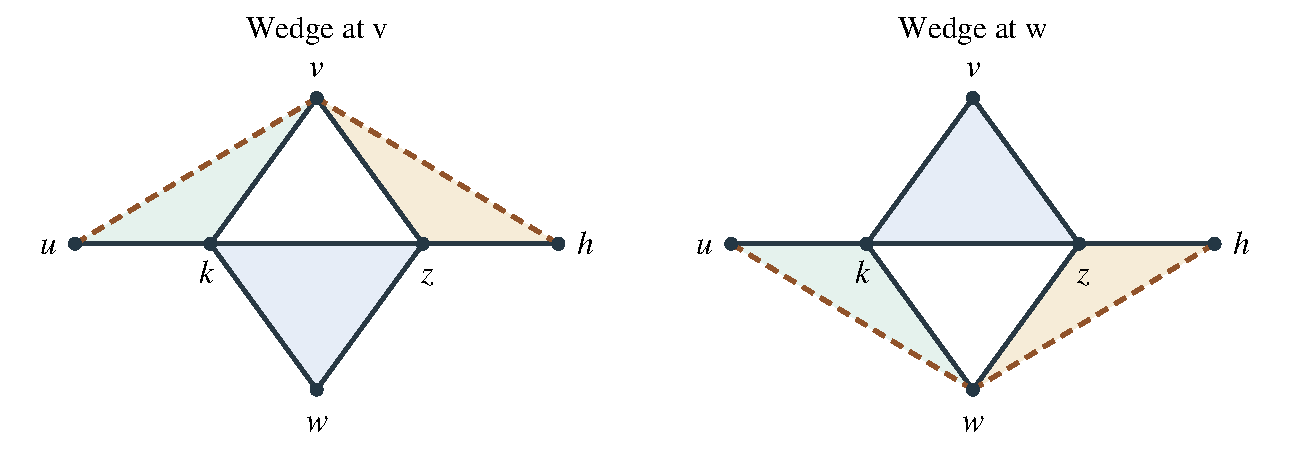
\includegraphics[width=.92\linewidth]{figures/crossing-hinge.pdf}
\caption{The seven solid edges are the same in both panels. Adding the dashed wedge at $v$ gives $kuv,hvz,kwz$. Adding the dashed wedge at $w$ gives $kuw,hwz,kvz$. The three shaded triangles in either panel partition all nine edges. The shared edge $uh$ stays outside both decompositions.}
\end{figure}

\subsection{6. Proof of the statistics theorem}\label{proof-of-the-statistics-theorem}

The same assignment must approximate the prescribed counts on the whole graph and on its original core. We choose the host pools before deletion so that a Pasch can be counted in the block that owns its bases.

\textbf{Construction of the initial pools.} Use the two orders of Lemma 5 for the 54 role types. For each of the 66 remaining types take a separate block on the original core, \(K_{t,t}\) for two distinct roles and \(K_t\) for one role, with \(Kt\) hosts each. The original core and these two sets of hosts use at most \([15+K(1296j+66)]t\) vertices. Use this bracket in place of \(B_j\) in Section 4. Its order is still \(\Theta_p(j)\), so the rounding estimate and (10) still apply.

Each of the three color classes has \(d_0=5t\) original vertices. Let \(w\) be the largest multiple of \(d_0\) at most \(p^2 n/64\), and take \(|W|=w\). Since \(t=\Theta_p(n/\sqrt{\log n})\), we have \(w\sim p^2 n/64\). Divide the remaining host budget into four equal pools, up to at most three extra hosts seeing just \(W\). Each pool contains at least \(n/8\) hosts for large \(n\). One sees just \(W\), and each of the other three sees \(W\) and one original color class. As before, all original hosts also see \(W\).

Divide \(W\) into slices of \(d_0\) vertices. In the pool for color \(i\), assign a disjoint set of \(\lceil(1+\eta)d_0/p\rceil\) hosts to each slice for its \(K_{d_0,d_0}\) of requests to \(V_i\). The number required is \(((1+\eta)/p+o(1))w<n/8\) for small fixed \(\eta\). Take \(\lceil(1+\eta)w/p\rceil<n/8\) hosts in the fourth pool for the terminal block \(K_w\). For the original blocks use the prescribed subpool of Theorem 1 inside the \(Kd\) available hosts. When prefix pairs reuse a pool in Lemma 5, the same subpool serves their disjoint vertex sets. All these choices precede the deletions.

\textbf{Lemma 7 (localization of Pasch configurations).} With the initial pools just described, every Pasch configuration of designated candidates belongs to exactly one auxiliary block, with secondary blocks restricted to their owned bases. The conclusion also holds for every subfamily of the candidates, in particular for any post-deletion assignment.

\emph{Proof.} \emph{Terminal and mixed blocks.} Each of the four triangles has one host. Every vertex of a Pasch appears twice, so the four host occurrences give exactly two hosts. The two triangles at either host have disjoint bases, since otherwise they would share a crossing edge. The four core vertices therefore occur once at each host. The two matchings on these four vertices share no base, since no two triangles in a Pasch share an edge. Their union is a four-cycle. A mixed host uses bases between one slice of \(W\) and one \(V_i\). A second host using the same four vertices must be from that same mixed block: its alternative matching either uses mixed pairs again, or would require one host to use both a \(W\)-internal and an original-internal pair. No host is assigned both kinds. A Pasch on four vertices of \(W\) lies in the terminal block.

\emph{Original role pairs.} In the original core, a host using a repeated role forces all four vertices into that role. For two distinct roles, a matching using two within-role pairs would require one host to serve both roles internally. Thus the second host must serve the same role pair as the first. For the 66 types this already locates the block.

\emph{Role pairs using the two orders.} In one of the 54 other types write the bases at the first host as \(u_1v_1,u_2v_2\), and those at the second as \(u_1v_2,u_2v_1\). In any coordinate observed by the first host, equality of the two midpoint coordinates gives \(u_1+v_1=u_2+v_2\). The two crossed differences are therefore equal, and their common value is the average of the two direct differences. If the first host fails at an earlier original coordinate than the second, (9), after division by the role distance, puts the crossed direction outside \(S_m\). Both retained crossed bases must lie inside \(S_m\) in every original coordinate preceding their failure. This includes the penultimate coordinate for a secondary block. Thus the two failure coordinates coincide.

The two hosts now observe the same prefix. There we have both \(u_1+v_1=u_2+v_2\) and \(u_1+v_2=u_2+v_1\). Subtraction gives \(2(v_1-v_2)=0\). Since \(m\) is odd, the two \(v\) prefixes agree, as do the two \(u\) prefixes. The failed direction fixes the class, and the common midpoint fixes the center prefix. All four triangles belong to the same block. The argument used only ownership and the initial permitted incidences, so it applies both to a realized Pasch and to a summand of \(P_\lambda\). A base has a unique owner, so the common block is unique. \(\square\)

\emph{Proof of Theorem 2.} The least side size of an original block is at least \(m^2\), and there are \(O(n^2)\) nonempty blocks. For fixed \(\eta\) the probability that any block fails Theorem 1 is at most \(O(n^2)\exp(-\Omega_{p,\eta}(m^{2/3}))=o(1)\). Within every successful block choose the factors and the corrected positive weights \(\mu\) of Theorem 1. We apply T+ to each full auxiliary block. In a secondary block we discard every triangle whose base belongs to a primary block, removing both crossing incidences of that triangle from the secondary support. The retained triangles determine the final support of that block. In all other blocks every incidence selected by the factors is used exactly once. Distinct blocks with a common host have disjoint core endpoints, and all retained bases have a unique owner. This gives one complete assignment. Surviving crossing edges outside its selected support remain available as individual edges in the partition calculation (7). Identity (7) and the neighbor count in \(W\) prove (5) and (6) for this choice of witnesses as well.

\textbf{Replacing the random target by the prescribed one.} Consider any full auxiliary block of side size \(d\) and prescribed pool size \(r\). Extend \(\mu\) by zero to discarded candidates and put

\[\widetilde\lambda_T=\frac{\mathbf1_{\{\text{both incidences of }T\text{ survive}\}}}{p^2r}.\]

On triangles retained by the factors the starting weight in Theorem 1 is \(1/a_h\) or \(1/(a_h-1)\). The denominator is \(d^2/r+O_p(1)\) in either case. Since \(pr/d=1+\eta+O_p(1/d)\), this starting weight differs from \(1/(p^2r)\) by \(O_p((\eta+1/d)/d)\). The correction to obtain \(\mu\) is \(O_p((\eta+d^{-1/3})/d)\). There are \(O_p(d^3)\) candidates. The factors discard \(O_p(\eta d^2)\) surviving incidences for large \(d\), each in \(O(d)\) candidates of weight \(O_p(1/d)\). Consequently

\[\sum_T|\mu_T-\widetilde\lambda_T|
     =O_p\big((\eta+d^{-1/3})d^2\big).
\tag{13}\]

This bounds the change of the target for every \(|f|\le1\). For Pasch, expand a difference of two products by changing one of the four factors at a time. A fixed triangle lies in \(O_p(d^3)\) candidate configurations (choose the second host and the two additional core vertices), and each of the other three weights is \(O_p(1/d)\). Thus a constant times (13) also bounds the change of the Pasch target.

The expectation of \(\widetilde\lambda_T\) is \(1/r\). The four triangles of a Pasch use eight distinct crossing edges, so the expectation of their product of comparison weights is \(p^8/(p^2r)^4=r^{-4}\). In this way (1) is the expectation of each comparison target. Changing one incidence affects \(O(d)\) triangles and \(O_p(d^4)\) candidate Pasch configurations, changing either target by \(O_p(1)\). There are \(O_p(d^2)\) independent incidence trials in the block. The bounded-differences inequality {[}9{]} gives deviation at most \(d^{5/3}\) except with probability \(2\exp(-\Omega_p(d^{4/3}))\) per target. A union bound suffices for all the prescribed tests and blocks.

\textbf{The original core.} Put \(a=\lfloor j/2\rfloor\) and \(\rho_m=|S_m|/m^2\). The region defining \(S_m\) in {[}1, §6{]} misses the square \([0,1/2)^2\). On the odd grid that square contains \(((m+1)/2)^2\) points, so \(\rho_m\le 3/4\). Call a primary block early if its first failure occurs at coordinate \(i\le a\). Its side length is \(m^{2(j-i)}\ge\sqrt t\). We include the 66 unrestricted role types among the large blocks as well. Those blocks have side \(t\) and require no cropping.

For a fixed pair of distinct roles, each direction occurs on exactly \(t\) bases, one for each starting position. In one of the 54 restricted types the early blocks therefore contain exactly \(t^2(1-\rho_m^a)\) bases, each once. The remaining primary blocks have at most \(t^2\rho_m^a\) bases. In the secondary order, even \emph{before} cropping, the first \(j-2\) original coordinates must pass. Hence its full blocks have at most \(t^2\rho_m^{j-2}\) bases in total, since the last coordinate and its class give at most one block per base. For \(j\ge4\) this is at most \(t^2\rho_m^a\). Summing over the 54 types bounds the late and secondary bases with multiplicity by \(108t^2(3/4)^a=o(t^2)\).

On each of these smaller blocks we ask T+ for the Pasch count alone, at fixed accuracy, say one. There are \(O_p(d^6)\) candidate configurations, each of fractional weight \(O_p(d^{-4})\) in the seed, so the realized count is \(O_p(d^2)\). The initial target obeys the same bound. Cropping decreases both counts. For a test of absolute value at most one, each base accounts for at most one unit in the assignment and in the initial target. Lemma 7 ensures that no additional Pasch contribution crosses a block boundary. Thus the smaller blocks together cost \(o(t^2)\) in either comparison, uniformly in the tests.

\textbf{One choice of decompositions.} Apply T+ in each early, unrestricted, mixed and terminal block to all restrictions of the given tests and to Pasch together. In these blocks \(N\ge d\ge\sqrt t\), so for fixed \(q\) we have \(n^q\le N^{2\lceil q\rceil+2}\) for sufficiently large \(n\), using \(t=\Theta_p(n/\sqrt{\log n})\). The concentration bound above holds jointly over the polynomially many blocks and tests. On this event the sum of the target comparison and decomposition errors in each such block is at most \(O_p((\eta+\varepsilon+d^{-1/3})d^2)\) for fixed \(\eta,\varepsilon\). Each term is charged to that block once. The original blocks have \(\sum d^2=O(t^2)\), counting the full secondary blocks. Across the whole construction \(\sum d^2=O_p(n^2)\), since a full block contains \(\Theta(d^2)\) bases. Summing first on the original blocks and then on all blocks gives normalized errors \(O_p(\eta+\varepsilon)+o(1)\) on both scales for the same assignment.

To obtain one sequence of witnesses, take \(\eta_i,\varepsilon_i\downarrow0\) satisfying Theorem 1. At stage \(i\) allow up to \(n^i\) tests. Choose \(n_i\) increasing so that beyond \(n_i\) the relevant block orders meet the corresponding T+ thresholds, both remaining normalized errors are at most \(1/i\), and the failure probability for any given family of this size is at most \(1/i\). The estimates use only the number and uniform bound of the tests. Use the stage-\(i\) pools for \(n_i\le n<n_{i+1}\). Every fixed \(q\) is eventually covered. The witnesses and reference weights are independent of the choice of tests. Once the tests are given, their target values are determined before deletion. The assignment may depend on both. This proves (2) and (3).

\textbf{The two Pasch counts.} In a bipartite block the number of four-cycles of bases is \(\binom d2^2\). In a clique block it is \(3\binom d4\). For any such cycle the two alternating matchings may be given distinct hosts in \(r(r-1)\) ways, each of weight \(r^{-4}\). Thus the initial Pasch target per block is its number of four-cycles times \((r-1)/r^3\). This is \(O_p(d^2)\), or a bounded amount per base. There are \(O(t^2+wt)=o(n^2)\) original and mixed bases, with the same order bound counting auxiliary copies. The terminal clique supplies the leading term. There \(r\sim w/p\), so

\[3\binom w4\frac{r-1}{r^3}
   =\frac{p^2w^2}{8}+o(n^2)
   =\frac{p^6}{32768}n^2+o(n^2).\]

On the original core the 105 distinct pairs of roles consist of 51 unrestricted types and 54 restricted types. The large bipartite blocks have \([51+54(1-\rho_m^a)]t^2=(105+o(1))t^2\) bases altogether. There are also 15 unrestricted clique blocks of order \(t\). Uniformly on the large blocks, \(d\to\infty\) and \(r/d\to1/p\) along the chosen sequence. Thus \(\binom d2^2(r-1)/r^3=(p^2/4+o(1))d^2\) for a bipartite block, whereas \(3\binom t4(r-1)/r^3=(p^2/8+o(1))t^2\) for each clique block. The smaller blocks contribute \(o(t^2)\). Adding the targets gives \[P_{\lambda,U}=\left(105\,\frac{p^2}{4}+15\,\frac{p^2}{8}\right)t^2+o(t^2)
=\frac{225p^2}{8}t^2+o(t^2).\] Equations (2) and (3) transfer the two target counts to \(\mathcal D\), proving (4). \(\square\)

Throughout the paper \(p\) is fixed as \(n\) grows. The list-mass margin in Theorem 4 and the common-neighbor densities in Theorem 1 are obtained with \(p\) fixed. For \(p=p(n)\) tending to zero, it remains to determine how rapidly \(p\) may decay while preserving a lower bound of the order in (5) and a complete post-deletion assignment with high probability.

\subsection{7. Formalization}\label{formalization}

The Lean 4 supplement of November 24, 2026 is available at \url{https://raw.githubusercontent.com/jtraverso/split-clique-partition-gap/main/preprints/SPLITGAPIII/05_formalization/split-gap-iii-lean-v0.4.zip}. The PDF edition also includes the archive as an attachment. Its SHA-256 is \nolinkurl{f5e51ff6a95f04688e92e5c291528ba14c689acda765282cde10c5a4c55cba46}. The table gives the principal declarations in the namespace \texttt{SplitGapIII}. The archive includes the sources, pinned dependencies and recorded axiom reports for 77 declarations. The sharp threshold in Theorem 4, the high-probability construction of a common support satisfying H1--H4 in Theorem 1, and the two-scale asymptotics in Theorem 2 are established analytically in Sections 2, 5, and 6, respectively.

{\def\LTcaptype{none} % do not increment counter
\begin{longtable}[]{@{}
  >{\raggedright\arraybackslash}p{(\linewidth - 2\tabcolsep) * \real{0.5000}}
  >{\raggedright\arraybackslash}p{(\linewidth - 2\tabcolsep) * \real{0.5000}}@{}}
\toprule\noalign{}
\begin{minipage}[b]{\linewidth}\raggedright
Lean declaration
\end{minipage} & \begin{minipage}[b]{\linewidth}\raggedright
Scope
\end{minipage} \\
\midrule\noalign{}
\endhead
\bottomrule\noalign{}
\endlastfoot
\nolinkurl{split_gap_recovery_all_orders}, \nolinkurl{all_orders_error_tendsto_zero} & Gap recovery at all sufficiently large orders for the construction with extra host copies. \\
\nolinkurl{hosted_clique_deficit_mem}, \nolinkurl{selected_hinge_condition} & Integer correction in the selected clique lattice and H4 from counts of ordered six-vertex completions. \\
\nolinkurl{hosted_pasch_one_block} & Localization of a hosted Pasch from the ownership conditions on its four candidate triangles. \\
\nolinkurl{selected_decomposition_with_reference_targets} & One T+ decomposition for all tests and Pasch on a selected support, given the seed, physical hypotheses and reference-target error bounds. \\
\end{longtable}
}

\subsection{Appendix A. Proof of Proposition 6}\label{appendix-a.-proof-of-proposition-6}

\emph{Proof.} For each of the 54 role types and each coordinate \(i\) and class \(C\), take the cylinder of directions defined by \(u_i\in C\), leaving all other coordinates free. Use two hosts per center with the neighborhoods of Lemma 5. For a fixed center coordinate \(z_i\) this gives a group of \(2s\) identical hosts. Assign each required direction to its first failed coordinate, its class there and the corresponding midpoint coordinate. Each full center accounts for a matching, since its two endpoints determine each other. The \(s\) full centers in the group therefore give a bipartite request graph of maximum degree at most \(s\). Its pairs retain at least \(2s-2\lfloor s/2\rfloor\ge s\) common hosts each. Galvin's list edge-coloring theorem {[}4{]} assigns them properly. For each of the 66 remaining types, we allocate \(2t\) hosts adjacent to every vertex of the corresponding role or pair of roles, where \(t=m^{2j}\). At least \(t\) common hosts survive on each pair since \(s\le t\). Galvin applies between distinct roles and the bound \(\chi'_\ell(K_t)\le t\) of Häggkvist and Janssen {[}5{]} applies within one role.

Including the original core, these groups use at most \((147+2592j)t\le(255+2880j)t\le n/25\) vertices by {[}1{]}. As in {[}2, Proposition 6a{]}, add \(W\) of size \(w\) and three families of \(w+v\) hosts seeing \(W\cup V_i\). This uses at most \(n/25+4w+3v\le24n/25+4\) vertices. The remaining places suffice for \(r\) additional hosts per family. Any final padding hosts see only \(W\). We may connect every original host to \(W\) as well.

Write \(b=\lfloor(v+r)/2\rfloor\). Each mixed pair from \(W\) to \(V_i\) retains at least \(w+v+r-2b\ge w\) common hosts in its own family. Since \(w\ge v\), Galvin colors the mixed pairs there. At each vertex of \(W\) these three colorings use at most \(v\) hosts altogether, one for each original vertex. For a pair within \(W\), discarding the missing incidences and every host already used at either endpoint leaves at least

\[3(w+v+r)-2b-2v\ \ge\ 3w+2r\ \ge\ w\]

available hosts. The list bound for \(K_w\) completes the assignment. Its original, mixed and internal pairs have disjoint crossing incidences by construction, so (7) applies before and after deletion. \(\square\)

\subsection{Appendix B. The cut estimate for the selected factors}\label{appendix-b.-the-cut-estimate-for-the-selected-factors}

On one core side of size \(d\), write \(k=d\) for a bipartite block and \(k=d-1\) for a clique block. The required core degrees are \(k\) and the required host degrees sum to \(kd\). Put \(\bar a=kd/r\). In the bipartite case \(|a_h-\bar a|\le1\). In the clique case choosing the two bracketing even values gives \(|a_h-\bar a|\le2\) and the prescribed total is attainable because \(kd\) is even. In particular \(a_{\min},a_{\max}=\Theta_p(d)\) for all sufficiently small fixed \(\eta\) and large \(d\).

Let \(x=|X|\), \(y=|Y|\), \(b=\min(x,y)\), and let \(T=kx+\sum_{h\in Y}a_h-kd\) be the cut demand. A cut with \(T\le0\) holds automatically. If \(T>0\), expressing it once in terms of \(Y\) and once in terms of its complement gives \[a_{\min}(r-y)<kx,\qquad k(d-x)<a_{\max}y .\] Consequently \(r-y\le C_px\) and \(d-x\le C_py\). If \(b=x\), we choose \(b\) core vertices and at most \(C_pb\) omitted hosts. If \(b=y\), we choose \(b\) hosts and at most \(C_pb\) omitted core vertices. Either list of choices has length at most \((d+r+1)^{(C_p+1)b+2}\), using an ordered list padded by a blank symbol. Also \(\max(x,y)=\Omega_p(d)\) since \(d\le x+C_py\). Hence \(xy=\Omega_p(db)\) and \(b\ge1\).

Write \(u=x/d\) and \(v=y/r\). The deviations of the \(a_h\) from \(\bar a\) sum to zero, so \(|\sum_{h\in Y}(a_h-\bar a)|\le2\min(y,r-y)=O_p(b)\). Since \(pr\ge(1+\eta)d\ge(1+\eta)k\), subtraction from the binomial mean gives \[pxy-T\ \ge\ kd(1-u)(1-v)+\eta kd\,uv-O_p(b).\] Here \(kd\,uv=(k/r)xy=\Theta_p(xy)\). For fixed \(\eta>0\), the rounding term is \(O_p(xy/d)\), so the mean exceeds the demand by at least a fixed positive fraction of \(pxy\) for large \(d\). Chernoff's inequality bounds the probability of failing this cut by \(\exp(-c_{p,\eta}db)\). The probability of any failure is at most \[\sum_{b=1}^{d}\exp\big(C'_pb\log d-c_{p,\eta}db\big)
       =\exp(-\Omega_{p,\eta}(d)).\] The same bound holds on either side of a bipartite block. Taking the union of the two failure events allows the two factors to use the same prescribed sequence of host degrees.

\subsection{Acknowledgments}\label{acknowledgments}

The author is deeply grateful to his wife María Paz and his children Lucas, Juan Cristóbal, Francisca, Raimundo and Benjamín for their love, patience and support.

\subsection{Use of artificial intelligence and computational tools}\label{use-of-artificial-intelligence-and-computational-tools}

Claude, by Anthropic, and ChatGPT/Codex, by OpenAI, were used to explore and check arguments and to prepare the manuscript.

The author remains responsible for the arguments, citations, code and presentation. No AI system is listed as an author.

\subsection{References}\label{references}

{[}1{]} J. P. Traverso Gianini, \emph{Nearly Quadratic Additive Gaps for Edge-Clique Partitions of Split Graphs}, preprint 1.0 (2026), Lemma 2.1 and §§4--6. \url{https://doi.org/10.5281/zenodo.24408988}

{[}2{]} J. P. Traverso Gianini, \emph{Stability of the Clique Partition Gap in Split Graphs}, preprint 1.0 (2026), Theorem 1, Lemma 2 and Proposition 6a. \url{https://doi.org/10.5281/zenodo.24452724}

{[}3{]} M. Bonamy, M. Delcourt, R. Lang and L. Postle, \emph{Edge-colouring graphs with local list sizes}, Journal of Combinatorial Theory, Series B \textbf{165} (2024), Theorem 6. \url{https://doi.org/10.1016/j.jctb.2023.10.010}

{[}4{]} F. Galvin, \emph{The List Chromatic Index of a Bipartite Multigraph}, Journal of Combinatorial Theory, Series B \textbf{63} (1995), 153--158. \url{https://doi.org/10.1006/jctb.1995.1011}

{[}5{]} R. Häggkvist and J. Janssen, \emph{New bounds on the list-chromatic index of the complete graph and other simple graphs}, Combinatorics, Probability and Computing \textbf{6} (1997), 295--313, Theorem 1.1. \url{https://doi.org/10.1017/S0963548397002927}

{[}6{]} J. P. Traverso Gianini, \emph{Triangle decompositions III: Physical typed absorption and prescribed statistics}, preprint 1.0 (2026), Theorems T and T+, §§2.1--2.3. \url{https://doi.org/10.5281/zenodo.23867836} \url{https://github.com/jtraverso/physical-typed-absorption}

{[}7{]} J. Balogh, J. He, R. A. Krueger, T. Nguyen and M. C. Wigal, \emph{Clique covers and decompositions of cliques of graphs}, Advances in Combinatorics (2026), Paper No.~9, Theorem 1.10. \url{https://doi.org/10.19086/aic.2026.9}

{[}8{]} V. Jain and H. T. Pham, \emph{Optimal thresholds for Latin squares, Steiner triple systems, and edge colorings}, Proceedings of the 2024 Annual ACM-SIAM Symposium on Discrete Algorithms, 1425--1436. \url{https://doi.org/10.1137/1.9781611977912.57}

{[}9{]} C. McDiarmid, \emph{On the method of bounded differences}, in \emph{Surveys in Combinatorics, 1989}, London Mathematical Society Lecture Note Series 141, Cambridge University Press (1989), 148--188. \url{https://doi.org/10.1017/CBO9781107359949.008}

{[}10{]} P. Keevash, \emph{The optimal edge-colouring threshold}, arXiv:2212.04397. \url{https://arxiv.org/abs/2212.04397}

\end{document}
